\chapter{Introduction}
\label{chap:intro}

\section{Research Motivation}
Alzheimer's disease (AD) is currently the leading cause of dementia worldwide, progressively eroding memory, cognitive reasoning, and functional autonomy in daily living \cite{cdc2024alzheimers}. Prior to developing overt dementia, the majority of patients pass through a pivotal intermediate stage known as \emph{mild cognitive impairment} (MCI): at this stage, memory or specific cognitive faculties have declined noticeably relative to age-normative expectations, yet individuals retain independence across most basic daily activities and primarily experience difficulties with complex cognitive tasks \cite{jack2018niaaa}. Notably, the clinical trajectories of individuals with MCI are remarkably heterogeneous: some patients convert rapidly to dementia within a short period, whereas others remain clinically stable for many years or even exhibit cognitive improvement \cite{petersen2018mci}. Motivated by this clinical reality, this thesis addresses a core research question: \emph{Given the longitudinal clinical history of an individual with MCI, can we accurately rank whether that patient faces an earlier or later risk of progression?}

A single scan can support risk prediction, but measuring within-person anatomical change requires observations at more than one time point. Indeed, a single structural brain magnetic resonance imaging (MRI) scan only reflects anatomical morphology on the exact day of acquisition, much like a static photograph that cannot convey the velocity or trajectory of tissue degeneration. Conversely, tracking a sequence of repeated scans from the same individual over time provides the necessary foundation for a model to capture the rate of anatomical atrophy, such as the pace of hippocampal volume loss \cite{dong2021deepatrophy}. Crucially, in real-world clinical follow-up data, the time intervals between consecutive visits are not uniform but vary considerably across patients (Table~\ref{tab:baseline-characteristics}). Consequently, I employ a Time-Aware Long Short-Term Memory (T-LSTM) network, which incorporates the actual elapsed time intervals between consecutive visits directly into the recurrent state update equations \cite{baytas2017patient}.

Furthermore, at each clinical visit, this thesis does not rely solely on a single MRI modality but actively harnesses three deeply complementary sources of information:
\begin{enumerate}
\item \emph{3D structural magnetic resonance imaging (MRI)}: provides comprehensive anatomical coverage of the brain and captures macroscopic structural changes such as hippocampal atrophy or ventricular enlargement \cite{weiner2015impact}.
\item \emph{Radiomics features}: a collection of quantitative mathematical descriptors that directly measure spatial geometry, voxel intensity distributions, and the coarseness or fineness of brain tissue textures extracted from the MRI volume itself \cite{vangriethuysen2017computational}.
\item \emph{Clinical data}: quantitative scores from the Mini-Mental State Examination (MMSE) and the Clinical Dementia Rating (CDR) scale evaluating cognitive and functional decline \cite{folstein1975mmse,morris1993cdr}.
\end{enumerate}

Although these three data sources reflect the pathological state of the same individual from complementary perspectives, they differ fundamentally in physical nature, representational dimensionality, and signal-to-noise characteristics. Consequently, the strategy used to fuse them plays a decisive role in determining the model's prognostic accuracy. Specifically, in the study serving as the direct reference baseline for this thesis, Aghajanian et al. (2025) combined a convolutional neural network (CNN), principal component analysis (PCA), a T-LSTM, and an attention mechanism over longitudinal MRI sequences to estimate progression risk under a Cox proportional hazards survival framework \cite{aghajanian2025longitudinal}. However, under their exact T-LSTM with attention configuration (Table~2 of their paper), concatenating gray-matter radiomics features with CNN features caused the mean concordance index (C-index) to decrease slightly from 0.85 to 0.84 on the validation set and from 0.91 to 0.90 on the test set; for this reason, the authors excluded radiomics from their final model \cite{aghajanian2025longitudinal}. This empirical finding raises a compelling scientific question: \emph{Could the apparent lack of benefit from radiomics stem from the fact that simple feature concatenation fails to exploit cross-modal interactions across data sources?}

To address this question, this thesis inherits the prognostic task formulation and reference data framework of Aghajanian et al., but fundamentally redesigns the multimodal fusion mechanism. Rather than merely concatenating feature vectors side by side, I explicitly model bilinear interactions between pairs of modalities. Specifically, given three sources---MRI (M), radiomics (R), and clinical scores (C)---there are three candidate pairwise interactions: MRI--Radiomics (MR), MRI--Clinical (MC), and Radiomics--Clinical (RC). To thoroughly mitigate the risk of parameter explosion when computing cross-products on a modest medical cohort, each bilinear interaction layer is tightly compressed via \emph{low-rank Canonical Polyadic (CP) tensor decomposition} \cite{kolda2009tensor,liu2018lowrank}, and the resulting interaction signals are routed back to the original modality representations through dynamically gated residual connections. In particular, recognizing that radiomics features are derived directly from the MRI scan itself, I propose a streamlined architecture termed \textbf{RC-Free Pairwise Fusion (RC-Free)}: positioning MRI as the central hub connecting the MR and MC pairs while deliberately omitting the direct RC interaction. The validity and effectiveness of this architectural choice are rigorously verified through controlled empirical comparisons against all seven pairwise interaction topologies in Section~\ref{sec:new-topology}.

\section{Problem Formulation}
This thesis addresses the problem of building a deep survival model to rank progression risk among individuals with MCI using data from the Alzheimer's Disease Neuroimaging Initiative (ADNI) \cite{weiner2015impact}. The study cohort comprises 359 participants who completed three MRI scans within 18 months of their baseline visit; each scan is synchronously paired with its corresponding whole-brain radiomics feature vector and clinical assessment scores. The three scan dates $s_1<s_2<s_3=p\leq L$ form a longitudinal observation sequence with subject-specific inter-visit time intervals. From this sequence of three clinical visits, the proposed method estimates a scalar log-risk score $\eta_i\in\mathbb R$ for each individual to rank future cognitive decline risk: participants assigned a higher $\eta_i$ are predicted to experience earlier progression.

\begin{figure}[H]
\centering
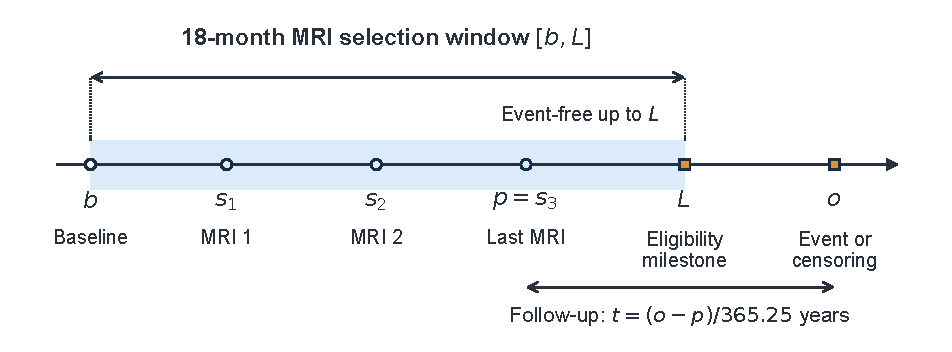
\includegraphics[width=\textwidth]{image_en/mci-progression-timeline.pdf}
\caption{Timeline of the longitudinal MCI progression prediction task}
\label{fig:problem-timeline}
\end{figure}

Figure~\ref{fig:problem-timeline} visually illustrates the temporal axis of the problem, clearly distinguishing the input observation window (three scans acquired at or before the cohort eligibility milestone $L$, defined as the baseline visit date plus 18 calendar months) from the post-$L$ clinical outcome follow-up period. To quantify cognitive and functional decline accurately, this thesis utilizes two well-established clinical rating scales:
\begin{enumerate}
\item \emph{MMSE (Mini-Mental State Examination)}: a 0-to-30 point scale evaluating global cognitive function, where lower scores indicate more severe cognitive impairment \cite{folstein1975mmse}.
\item \emph{CDR-global (global Clinical Dementia Rating)}: categorizes dementia severity into five levels---0 (normal), 0.5 (very mild dementia), 1 (mild), 2 (moderate), and 3 (severe)---according to the standardized scoring rules established by the scale's developers \cite{morris1993cdr,knightcdrscoring}.
\end{enumerate}

Inheriting the clinical convention of Aghajanian et al. \cite{aghajanian2025longitudinal}, a \emph{progression event} in this study is recorded at the first follow-up visit after milestone $L$ that satisfies either MMSE $<24$ or CDR-global $\geq1$. This constitutes a score-threshold-defined clinical event. Over long-term longitudinal follow-up, many participants withdraw from the study or reach the end of the observation period without ever crossing this threshold; consequently, their subsequent disease status remains unknown, except for the confirmed fact that they remained stable up to their last recorded visit. This statistical phenomenon is referred to as \emph{right-censoring}. Rather than forcing the task into a binary Yes/No classification paradigm (which would inevitably require discarding or mislabeling censored participants), this thesis formulates the problem within a \emph{survival analysis} framework to fully and equitably leverage both censoring status and actual follow-up duration.

Furthermore, from a methodological standpoint, a crucial detail in the time-axis definition must be noted: the survival model measures follow-up time starting from the third MRI scan date $p$, whereas the cohort inclusion criteria require participants to remain event-free through the 18-month milestone $L$. Whenever $p<L$, the interval between $p$ and $L$ is guaranteed to be event-free by virtue of the cohort selection rule itself, inducing \emph{immortal time bias} \cite{suissa2008immortal} if the model were interpreted as a prospective forecasting tool deployed immediately on scan date $p$. Accordingly, all empirical results in this thesis are carefully interpreted for the retrospective risk-ranking task among participants confirmed to have remained stable up to milestone $L$ (analyzed in detail in Sections~\ref{sec:study-design} and~\ref{sec:study-limitations}).

\section{Technical Challenges and Research Scope}
Developing a multimodal deep survival model over longitudinal medical sequences poses three primary technical challenges:
\begin{enumerate}
\item \emph{Balancing interaction expressiveness against parameter capacity}: Concatenating feature vectors introduces no additional parameters at the fusion step, but fails to explicitly construct second-order cross-products across modalities. Conversely, the outer product captures all bilinear interactions exhaustively, yet causes the weight count of the subsequent linear projection layer to grow multiplicatively with input and output dimensions \cite{zadeh2017tensor,liu2018lowrank}, easily triggering severe overfitting when the training set contains only 251 patients. While CP tensor decomposition substantially compresses the weight count via low-rank factorization \cite{kolda2009tensor,liu2018lowrank}, the trade-off between parameter compression and risk-ranking performance requires rigorous empirical validation.
\item \emph{Risk of representational redundancy across pairwise interactions}: Because radiomics features are mathematically extracted from the MRI volume itself, while clinical scores serve both as input predictors and as the basis for the outcome event criteria, maintaining all three pairwise interactions (MR, MC, and RC) simultaneously may inflate architectural complexity without contributing novel information. A systematic ablation study is therefore needed to identify the most compact and effective subset of pairwise interactions.
\item \emph{Training survival ranking models on high-memory 3D volumetric scans}: Because each participant is represented by three 3D brain volumes that consume substantial GPU memory, each training mini-batch can accommodate only a very small number of patients. At the same time, for the Cox partial log-likelihood loss to learn risk ranking, every training batch must contain at least one uncensored progression event paired with individuals who remained stable longer; under naive random batching, many mini-batches would lack any valid event pairs for gradient updates.
\end{enumerate}

To overcome these challenges, within the scope of this thesis, I conduct a controlled empirical investigation across three core architectural design choices. First, I perform a head-to-head comparison between traditional feature concatenation and bilinear outer-product fusion. Second, I quantify the parameter reduction and performance trade-off achieved by applying CP tensor decomposition. Third, I systematically evaluate all seven pairwise interaction topologies to validate the proposed RC-Free design. All primary experiments share an identical participant-level data partition and are repeated across three independent random initializations (seeds). Model performance is objectively evaluated using three complementary survival metrics: Harrell's concordance index (C-index), inverse-probability-of-censoring-weighted time-dependent ROC curves (IPCW-ROC), and Kaplan--Meier survival curves.

\section{Research Questions}
To guide the empirical evaluations in Chapter~\ref{chap:results}, I structure the investigation around five research questions (RQ1--RQ5), summarized in Table~\ref{tab:rq}, spanning temporal modeling (RQ1), multimodal fusion (RQ2--RQ3), CP compression (RQ4), and pairwise interaction pruning (RQ5).

\begin{table}[H]
\centering\footnotesize
\caption[Research questions and verification methodology]{Research questions and verification methodology.}
\label{tab:rq}
\setlength{\tabcolsep}{5pt}
\renewcommand{\arraystretch}{1.02}
\begin{tabularx}{\textwidth}{@{}Y Y@{}}
\toprule
\textbf{Research Question} & \textbf{Verification Methodology} \\
\midrule
\textbf{RQ1.} Do longitudinal multi-timepoint MRI scans provide superior risk discrimination compared with using only the final MRI scan? & Compare the \textit{Last-MRI} baseline against \textit{Longitudinal MRI + T-LSTM} and \textit{Longitudinal MRI + T-LSTM + Attention} to isolate the contribution of temporal dynamics. \\
\addlinespace[2pt]
\textbf{RQ2.} Does incorporating radiomics and clinical scores improve risk discrimination over using MRI alone? & Compare \textit{Longitudinal MRI + T-LSTM + Attention} against \textit{Three-Modality Concatenation} combining MRI, radiomics, and clinical features. \\
\addlinespace[2pt]
\textbf{RQ3.} Is pairwise bilinear interaction more effective than simple feature concatenation? & Compare Concatenation and Full Outer-Product across three random seeds under identical training protocols and matched initial weights for all shared modules. \\
\addlinespace[2pt]
\textbf{RQ4.} How many interaction-layer parameters does CP decomposition reduce, and how does it affect the C-index? & Compare Full Outer-Product and Full CP in terms of parameter counts across architectural scopes and validation C-index across three random seeds. \\
\addlinespace[2pt]
\textbf{RQ5.} Can redundant pairwise interactions be pruned while preserving risk discrimination performance? & Benchmark all seven CP topologies containing at least one active pairwise interaction (single-pair, two-pair variants including RC-Free, MR-Free, MC-Free, and three-pair Full CP). \\
\bottomrule
\end{tabularx}
\end{table}

\FloatBarrier
\Needspace{10\baselineskip}
\section{Thesis Contributions}
This thesis makes three primary contributions from both methodological and empirical perspectives:
\begin{enumerate}
\item \emph{An end-to-end multimodal longitudinal deep survival pipeline}: The thesis synchronously integrates 3D structural MRI volumes (encoded via a 3D ResNet-18 initialized from MedicalNet pretrained weights \cite{chen2019med3d}), whole-brain radiomics features, and clinical MMSE/CDR scores across three consecutive visits, combining a T-LSTM \cite{baytas2017patient}, an additive attention mechanism, and a Cox proportional hazards head to rank progression risk.
\item \emph{A gated CP pairwise fusion mechanism and the streamlined RC-Free topology}: The thesis replaces full outer-product projection layers with low-rank CP parameterization and routes interaction signals back to individual modalities via dynamically gated residual connections. By positioning MRI as the central hub connecting the MR and MC pairs, the proposed \textbf{RC-Free} architecture successfully eliminates the direct RC interaction while preserving all three input modalities.
\item \emph{A controlled empirical evaluation of parameter compactness and survival stratification}: CP decomposition reduces the parameter count of the three initial bilinear layers by \textbf{98.38\%} (Table~\ref{tab:interaction-parameters}), while the RC-Free topology saves an additional \textbf{15460 parameters} compared with Full CP. Evaluated on the same validation set across three random seeds, RC-Free achieves the highest mean C-index among all seven pairwise interaction topologies (\textbf{0.8347}, Table~\ref{tab:new-topology}) and yields statistically significant risk-group separation on Kaplan--Meier survival curves ($p=0.0134$ on the validation set; $p<0.001$ on the post-hoc test set, Table~\ref{tab:km-statistics}).
\end{enumerate}

The remainder of this thesis is organized into four sequential chapters. Chapter~\ref{chap:background} reviews the theoretical foundations of longitudinal data, survival analysis, and related literature. Chapter~\ref{chap:method} details cohort construction, multimodal preprocessing, the proposed RC-Free architecture, and the survival evaluation framework. Chapter~\ref{chap:results} presents the empirical experiments addressing RQ1 through RQ5 along with in-depth survival stratification analyses. Finally, Chapter~\ref{chap:discussion} discusses key architectural insights, outlines methodological limitations, proposes future research directions, and concludes the thesis.
